\documentclass{sigchi}

% Use this command to override the default ACM copyright statement
% (e.g. for preprints).  Consult the conference website for the
% camera-ready copyright statement.


%% EXAMPLE BEGIN -- HOW TO OVERRIDE THE DEFAULT COPYRIGHT STRIP -- (July 22, 2013 - Paul Baumann)
% \toappear{Permission to make digital or hard copies of all or part of this work for personal or classroom use is      granted without fee provided that copies are not made or distributed for profit or commercial advantage and that copies bear this notice and the full citation on the first page. Copyrights for components of this work owned by others than ACM must be honored. Abstracting with credit is permitted. To copy otherwise, or republish, to post on servers or to redistribute to lists, requires prior specific permission and/or a fee. Request permissions from permissions@acm.org. \\
% {\emph{CHI'14}}, April 26--May 1, 2014, Toronto, Canada. \\
% Copyright \copyright~2014 ACM ISBN/14/04...\$15.00. \\
% DOI string from ACM form confirmation}
%% EXAMPLE END -- HOW TO OVERRIDE THE DEFAULT COPYRIGHT STRIP -- (July 22, 2013 - Paul Baumann)


% Arabic page numbers for submission.  Remove this line to eliminate
% page numbers for the camera ready copy 

%\pagenumbering{arabic}

% Load basic packages
\usepackage{balance}  % to better equalize the last page
\usepackage{graphicx} % for EPS, load graphicx instead 
%\usepackage[T1]{fontenc}
\usepackage{txfonts}
\usepackage{times}    % comment if you want LaTeX's default font
\usepackage[pdftex]{hyperref}
% \usepackage{url}      % llt: nicely formatted URLs
\usepackage{color}
\usepackage{textcomp}
\usepackage{booktabs}
\usepackage{ccicons}
\usepackage{todonotes}
\usepackage{array}
\usepackage{subfigure}
\usepackage{multicol}

\usepackage{lipsum}
\usepackage{ragged2e}
\usepackage{float}
\usepackage{midfloat}
\usepackage{wrapfig}
\usepackage{makecell}
\usepackage{enumitem}

\newcounter{AppendixCounter}
\def\theAppendixCounter{\Alph{AppendixCounter}}

\long\def\createappendix #1{%
    \newpage%
    \refstepcounter{AppendixCounter}%
    \section*{Appendix \Alph{AppendixCounter}: #1}%
    \bigskip%
}

\hyphenation{Appendix}

\newenvironment{localsize}[1]
{%
  \clearpage
  \let\orignewcommand\newcommand
  \let\newcommand\renewcommand
  \makeatletter
  \input{bk#1.clo}%
  \makeatother
  \let\newcommand\orignewcommand
}

% llt: Define a global style for URLs, rather that the default one
\makeatletter
\def\url@leostyle{%
  \@ifundefined{selectfont}{\def\UrlFont{\sf}}{\def\UrlFont{\small\bf\ttfamily}}}
\makeatother
\urlstyle{leo}

% To make various LaTeX processors do the right thing with page size.
\def\pprw{8.5in}
\def\pprh{11in}
\special{papersize=\pprw,\pprh}
\setlength{\paperwidth}{\pprw}
\setlength{\paperheight}{\pprh}
\setlength{\pdfpagewidth}{\pprw}
\setlength{\pdfpageheight}{\pprh}

% Make sure hyperref comes last of your loaded packages, to give it a
% fighting chance of not being over-written, since its job is to
% redefine many LaTeX commands.
\definecolor{linkColor}{RGB}{6,125,233}
\hypersetup{%
  pdftitle={SIGCHI Conference Proceedings Format},
  pdfauthor={LaTeX},
  pdfkeywords={SIGCHI, proceedings, archival format},
  bookmarksnumbered,
  pdfstartview={FitH},
  colorlinks,
  citecolor=black,
  filecolor=black,
  linkcolor=black,
  urlcolor=linkColor,
  breaklinks=true,
}

% create a shortcut to typeset table headings
% \newcommand\tabhead[1]{\small\textbf{#1}}

% End of preamble. Here it comes the document.
\begin{document}

\title{StoryTime with Friends}

\numberofauthors{5}
\author{%
  \alignauthor{Ali Dehghan\\
    \affaddr{University of Victoria}\\
    \affaddr{Victoria, BC, Canada}\\    
    \email{dehghan1991@gmail.com}}
  \alignauthor{Brandon Mabey\\
    \affaddr{University of Victoria}\\
    \affaddr{Victoria, BC, Canada}\\   
    \email{brandonmabey@gmail.com}}
  \alignauthor{Courtnay Low\\
    \affaddr{University of Victoria}\\
    \affaddr{Victoria, BC, Canada}\\
    \email{cllow@uvic.ca}}
  \alignauthor{Sarah Warnock\\
    \affaddr{University of Victoria}\\
    \affaddr{Victoria, BC, Canada}\\  
    \email{srwarnock91@gmail.com}}
  \alignauthor{Shaquille Davis\\
    \affaddr{University of Victoria}\\
    \affaddr{Victoria, BC, Canada}\\    
    \email{shaq147@yahoo.com}}
}

\maketitle


\hyphenpenalty=400 %Try and prevent hyphenation


\begin{abstract}
 Friends are usually distributed over different locations. With the rise of collaborative technologies, people tend to use these collaborative tools for a variety of tasks, such as to connect, work, and stay in touch with friends and family. Since playing games is a common practice among friends, we want to allow Story Time, a collaborative story making game, to be played remotely and asynchronously with the support of computer technologies by translating and adapting its features to the new environment. To create such an application, we approached an iterative implementation methodology to finally achieve a minimum viable product for our application. In pursuit of this objective, we implemented two different prototypes of our game. This was followed by two evaluation sessions with a total of 9 volunteer participants. Through analysis of their responses to our interview questions along with an environmental study of their gameplay, we found that they enjoyed playing our game and provided insightful ideas for us to better adapt the game to the new environment. As the next step to our project, we will continue our implementation towards creating the MVP based on policies taken from the prototype evaluation result analysis.
\end{abstract}

\keywords{Computer supported collaborative work; Collaborative games; Game design; Word games
}

\section{Introduction}
We are implementing a Facebook web application named StoryTime with Friends, which is based off of a real life game called Story Time. Story Time is a mini-game within a drinking game known as Sociables \cite{sociablesrules}. Sociables is played by assigning a rule to each value within a deck of cards. The cards are then spread out in a circle where each player takes turns picking a card. Once a card is chosen the rule that is applied to that card must be played out. 

The Story Time rule is as follows: starting with the player who drew the card, create a story one word at a time. For example, the first player might start the story with ``Hello'', and the second player could continue the story with ``world'', making the story so far, ``Hello world'' and so on. An added element to the Story Time rule that we will not be implementing is one where a player must correctly recite the entire story thus far before adding a word of their own, otherwise they must drink. 

Currently this game is played synchronously and orally in a co-located setting. Our goal is to change its time-space matrix, making it possible for people to play it remotely and asynchronously by adapting the oral version to be computer supported. We aim to implement a game where players can create a funny and entertaining story which they will laugh at and enjoy reading

\subsection{One Word at a Time}
The version of Story Time that we are implementing is also extremely similar to a drama game called ``One Word At A Time'' \cite{dramaresource, izzyg, sociablesrules}. Unlike Story Time, One Word At A Time is not a drinking game; because of this it does not have the lose condition of being unable to recite the story to the current point. This makes the version being implemented into the digital domain more related to the ``One Word At A Time'' game than the Story Time rule from Sociables. However, note that the idea behind our game StoryTime with Friends was initiated from the rule within the drinking game Sociables.

Similar to ``One Word At A Time'', StoryTime with Friends does not impose the notion of winning or losing upon the players. Instead, the ability to maintain the spontaneity and flow of the story becomes the goal of the exercise \cite{improv.ca}. This means that there is no predefined end point or goal for which the game is caused to finish, unlike most games \cite{learn-canvas, badge-ville, makeschool}. 

\subsection{Online Versions of One Word at a Time}
Attempts at translating the game ``One Word At A Time'' to the digital space have created sub-par solutions in the past, usually resulting in failure. One solution generated by some people in order to recreate the game was to make a One Word At a Time subreddit, similar to an internet bulletin board or forum on the site reddit.com, \cite{reddit}. This internet space had become unused after just five sessions of the game.

Other attempts by people, such as the Clash of Clans Wikia forums, Crunchy Roll forums, and Battle.net forums have resulted in similar failures \cite{coc-wikia, crunchy-roll, battle.net}. Many other forums have had similar results in recreating the game \cite{minecraft, drummer-world, android}.

Surprisingly, some of these attempts to recreate the game on a forum board have worked. For example, the Nintendo Life forum has an instance of One Word At A Time left uncompleted with 4639 words present \cite{nintendo-life}. The Paizo forums has a game with 825 words \cite{paizo}.

\section{Background}
The game ``One Word At A Time'' is often played with five to ten players as part of an improvisation exercise, and is also called ``Word At a Time'', ``Sentence At a Time'', or ``Word At a Time Expert'' \cite{learnimprov}. Variations of the game support non-linear turn orders and the addition of full sentences to the story. Sometimes the participants in this game will act out the story as it is created. This often requires a large amount of coordination by the players as well as skill in non-verbal communication.

While the game's main focus is the ability to improve group coordination across the participating players, games played at a professional level, with an often modified set of game rules can lend itself to audience entertainment. It has been shown to be a popular form of entertainment for non-participants to spectate, as seen on the TV show ``Whose Line is it Anyway?'', where they play games such as ``Questions Only?'' and ``Questionable Impressions.'' \cite{whoseline}. The end result of either the professional spin-offs or amateur versions often lead to stories with comedic results.

\subsection{Related Games}
For the purposes of research, we are defining related games to be games that are translated from the co-located synchronous to remote asynchronous on Johansen's CSCW matrix \cite{cscw-matrix}. We will then use the MoCA framework \cite{MoCA} in order to evaluate these games.

\subsubsection{Next Sentence}
The most similar of these researched games is ``Next Sentence'', a mobile application available for Android and iOS, which displays these issues in its attempt to create a game similar to ``Word Spud'' in the remote asynchronous domain \cite{next-sentence, word-spud}. 

Next Sentence, created by Ripple Digital Publishing, is a cognitively distributed game where participants take turns adding a full sentence to a story given a few prior words in the current story\cite{next-sentence-how}. A player's turn starts with seeing the story title, and the last couple of words added, followed by making their own additions to the story. Being limited to only seeing the last sentence of a story creates a lack of consistency in the application, leading to a diminished ability for the user to distribute cognition, as defined in the paper by Hollan et al. \cite{distributed-cognition}. In addition, the player is not limited by a time limit or turn order, allowing any player using the Next Sentence app to add additional sentences to any story, even if they were the last player. This interface is shown in Fig.\@~\ref{fig:next-sentence:home-page} and \@~\ref{fig:next-sentence:game-play}. Each story may have unlimited players, but the story as a whole has a limited number of turns set during the creation of the game.


In terms of the MoCA framework, Next Sentence is asynchronous, remote, has few communities of practice, low nascence and is short-term. By design, however, it could have a large or small scale and both high and low turnover rates for any particular game.
\newline
\newline


\begin{figure}
\hfill
\subfigure[Next Sentence Home Page \label{fig:next-sentence:home-page}]{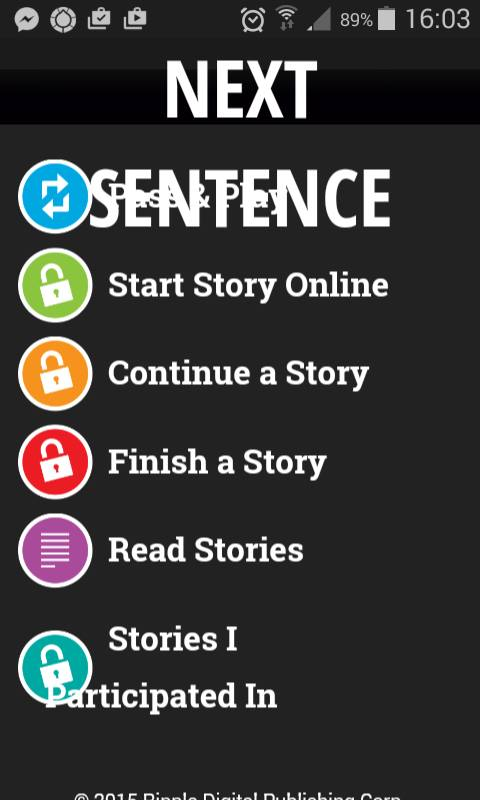
\includegraphics[height=6cm]{next_sentence.jpg}}
\hfil
\subfigure[Next Sentence Game Play Page \label{fig:next-sentence:game-play}]{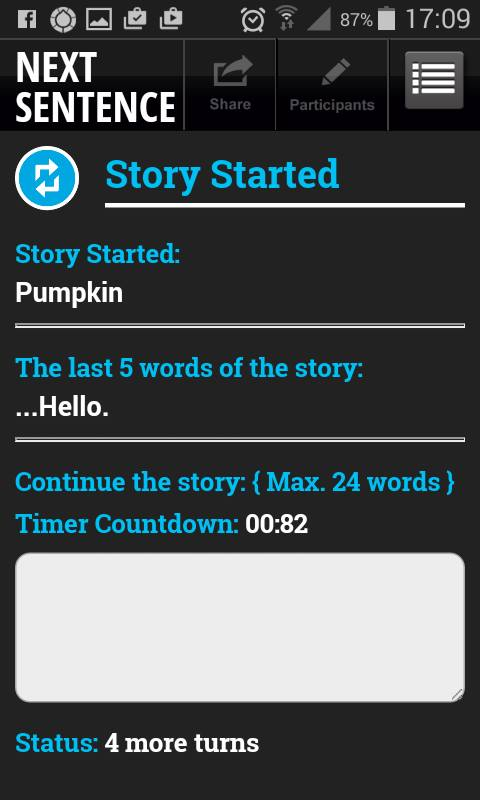
\includegraphics[height=6cm]{next_sentence_2.jpg}}
\hfill
\caption{Next Sentence Application Running on an Android Device}
\label{fig:next-sentence}
\end{figure}


\subsubsection{Words with Friends}
Another popular word game, ``Words with Friends'' available through Facebook and on mobile devices, was forced to undergo a similar change in Johansen's time-space matrix, from local and synchronous to asynchronous remote \cite{cscw-matrix, words-with-friends}. Words with Friends, which is very similar to the classic board game Scrabble, is a digital game taking place on a virtual board for two players \cite{words-with-friends-rules, scrabble}. The players take turns using lettered tiles to place on the board in a way that words form in horizontal and vertical configurations. Doing so, creates points based on the complexity of the word and rareness of the letters used, among other factors. The player with the most points at the end of the game is declared the winner \cite{words-with-friends-win}.

Words with Friends was able to overcome its transition on both Johansen's model and MoCA by making specific adaptations to the game to help support this transition. For instance, using all of one's word tiles at the same time is worth less in Words with Friends than with Scrabble due to the ability for the player to run anagram tools on their phone without their opponent's knowledge as would happen with Scrabble with the opponent watching you use an assistance tool \cite{wwf-vs-scrabble}. In addition, the user is prompted with game-specific context, such as the opponent they are facing, as this information is less accessible than it would be if it were to be played in the physical world. For example, the current opponent is displayed above the game board while the user is playing their turn \cite{words-with-friends-opponent}. Words with Friends, however, still suffers from reduced implicit context for the player as there is a reduced ability to read expressions from the opposing player due to the synchronous, remote, and digital nature of the application.

Based on the above explanation, Words with Friends is asynchronous, remote, has few communities of practice, is low nascence, short-term, small scale, and has a low turnover rate.
\newline


\subsubsection{Miscellaneous}
There are many additional, and similar games other than Words with Friends and Next Sentence which have undergone similar transitions from synchronous co-located to asynchronous remote. For instance, Draw Something is a digital implementation of Pictionary \cite{draw-something, draw-something-background}, which underwent similar transitions in the CSCW matrices. What's The Phrase is a personal game, which has many similarities to the televised Wheel of Fortune game show \cite{whats-the-phrase} and is another digital application located at a similar location as the others on the CSCW matrices. This shows that this transition in the matrices is a viable transition for many games currently played in person. While the above games represent a trend of transitions from synchronous co-located to asynchronous remote, there are numerous additional examples not included in this report to avoid unnecessary prolixity.

\section{Impact of Collaborative Games}
The article ``Collaborative Games: An Exploratory View for Instructional Designers'', written by Jason Drysdale of the University of Colorado, examines the value of collaborative games as team building and collaboration tools within team-based work environments.\cite{drysdale2011collaborative} It was found that more people identify themselves as gamers today than in the past. With 69 percent of heads of households and 97 percent of children playing video games. It is also noted that every one of four gamers is over 50 years old, with the average gamer being 30. Since the demographic of gamers has grown, video games have become more mainstream and can be a valuable medium for learning skills desired by most organizations if designed with collaboration in mind. Games provide many opportunities to develop and enhance teamwork and leadership skills; because of this many organizations use games as a way to provide content in a more fun and exploratory way to employees. There are three subgroups to collaboration within a collaborative game: cooperating, coordination, and co-creating. Our game, StoryTime with Friends has all three of these subgroups, making it a good candidate for enhancing team building and collaboration skills. Players must cooperate turn by turn in following a theme based on a provided title while co-creating a story. They do this by coordinating their personal input to the story to build off the input of the player before them.

\subsection{Related Literature}

\subsubsection{Distance Work}
In the workplace, distance plays a large factor in what makes a distributed team successful. Distributed teams are often made up of people from different backgrounds to produce a variety of ideas. \cite{distance} For the sake of our application, distance is one of the main factors of changing the time-space matrix of the game.

The common stressors that distributed teams face are:
\begin{itemize}[leftmargin=.5in, noitemsep]
\item Blind and invisible
\item Time-zone differences
\item Crossing institutional or cultural boundaries
\end{itemize}

The first stressor blind and invisible are when people on a team are invisible to those that are not at their location and must communicate and coordinate explicitly. StoryTime with Friends is played remotely with players contributing words to the story using their own device. They are able to see whose turn it is and how many people must take a turn before they can, but the activity of the other players are blind until the newly added words appear each time a player has finished their turn.

Due to the nature of the game being remote and asynchronous, playing with multiple people across different time zones may cause one to wait a long time until it is their turn again. In the full implementation of our application we will provide a time out feature, where a player's turn will be skipped if they are inactive for too long.

When crossing institutional or cultural boundaries in the workplace, conversational or decision-making practices and expectations may differ. This may also occur while playing StoryTime with Friends with people from different cultures. The story that has been written so far may not make much sense to someone, or certain words may have different meanings. 

\subsubsection{Distributed Cognition}
Distributed cognition is the psychological theory that an individual is not the only one containing knowledge, but that the individual's social and physical environment does as well. There are three ways that cognition can be distributed: 
	
\begin{enumerate}[leftmargin=.5in,noitemsep]
\item Cognitive processes may be distributed across the members of a social group.
\item Cognitive processes may be distributed in the sense that the operation of the cognitive system involves coordination between internal and external (material or environmental) structure.
\item Cognitive processes may be distributed through time in such a way that the products of earlier events can transform the nature of related events. 
\end{enumerate}

Our application touches on all the previously mentioned ways of distributing cognition. Since StoryTime with Friends users will be able to each add their own words to a shared story, cognition will be distributed across the members of the social group participating in the game. Also, because we are adapting the original game idea to be computer supported, the operation of the cognitive system will involve coordination between internal and external structures. The internal structure being the participating players individual contributions to the story, and the external structure being the computer supported environment supplied by the application that displays the end product of all those contributions. Lastly, the fact that users are able to see the story unfold as they wait for their next turn can change the words they choose to input when it is their turn once again. This ties into the third way that cognition may be distributed as listed above.


\section{Methodology}
We have conducted user studies that includes an interview and a demographic survey in order to collect data to be used for qualitative analysis. This section will thoroughly describe our StoryTime with Friends prototype, the user evaluation process, data analysis and conceptual design.

\subsection{Prototype}
Using the prototyping tool provided by www.proto.io, we created two prototypes of StoryTime with Friends for the purpose of conducting our prototype evaluation. There were 3 main objectives for the first round of interview (evaluation of prototypes):

\begin{enumerate}[leftmargin=.5in,noitemsep]
\item To watch the participants while playing the game and perform an environmental study.
\item To determine the enjoyability of our game.
\item To discover features and requirements for the game (number of players per story, time limits, number of input words per turn, etc).
\end{enumerate}

For the first prototype (Fig.\@~\ref{fig:prototype:non-tiled}), players are given the ability to contribute 4 or less words to the story during their turn. In the second prototype (Fig.\@~\ref{fig:prototype:tiled}), players are restricted to choosing 1 out of 6 tiles containing 4 or less words. The purpose of creating these two prototypes was to the determine which version the users preferred. The prototypes were played by our participants on one laptop, which was passed around after each turn. Due to unforeseen bugs when exporting our prototype onto a mobile device, we were forced to conduct the gameplay phase on a laptop. 

\begin{figure}
\hfill
\subfigure[Non-tiled Version \label{fig:prototype:non-tiled}]{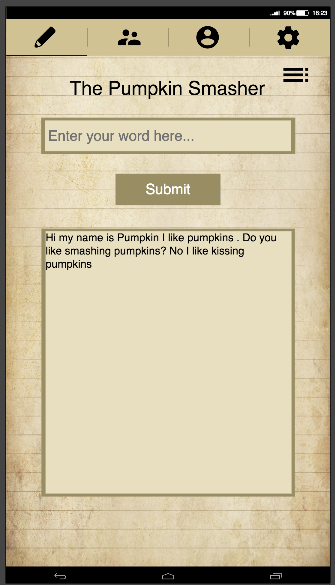
\includegraphics[height=6cm]{image01.png}}
\hfill
\subfigure[Tiled Version \label{fig:prototype:tiled}]{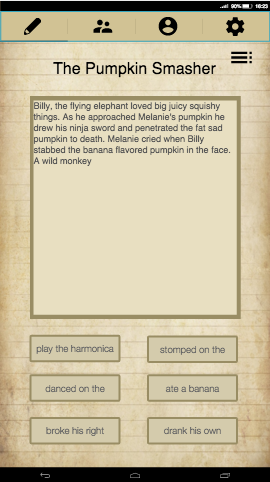
\includegraphics[height=6cm]{image02.png}}
\hfill
\caption{Prototype Used During User Test for StoryTime With Friends}
\label{fig:prototype}
\end{figure}



\subsection{Data Collection}
All the participants involved in the prototype evaluation are UVic undergraduate students between the ages of 18 to 24. We decided to select them as our target audience because university students typically have good background knowledge of various computer technology and games, and having a specific target audience for interviews generates more accurate and consistent results. Due to time constraints, limited accessibility, and indications in our ethics application, we were unable to involve a wider demographic of participants in our study. 

We conducted two prototype evaluation sessions, the first session consisted of four players, and the second session consisted of five players; both were conducted in the exact same manner. An explanation of our game was provided to the participants, followed by them filling out a simple multiple-choice demographic survey. After, we watched the participants as they used our prototypes. The first one they were given was the tiled version, followed by the non-tiled version. When they had finished playing, we interviewed the participants regarding their experience during the gameplay. The interviews were audio recorded and transcribed for further analysis.


\subsubsection{Demographic Questions}
We asked participants to answer our demographic questions through a questionnaire. The purpose of these demographic questions was to help us have a better understanding of our participants and analyze how their demographics may affect their gameplay or answers to the interview questions. All of these questions were about participants' experiences in playing different types of games.

The complete list of demographic questions are available in Appendix~\ref{apx:demographic}.


\subsubsection{Interview Questions}
Our interview questions were designed to target the three main objectives of the user evaluation that was previously described. 

The complete list of Interview questions is available in Appendix~\ref{apx:interview}.

\subsection{Data Analysis}
For privacy and ethical reasons, we replaced the names of our participants with code names after linking the data of each section (demographics, interview, and environmental study) together.
The audio recordings of the interviews were transcribed and placed in a shared document, and the summarized answers to the questions were placed in a table.

\subsubsection{Demographic Question Responses}
See Fig.\@~\ref{fig:demographics} for a summary of demographic questions responses. Although Considering the low number of participants in our prototype evaluation, these responses were not as helpful as what we where thinking of at the beginning, but they helped us to have a better understanding of the participants' backgrounds and therefore better design the rest of our study.

\begin{figure}
\centering
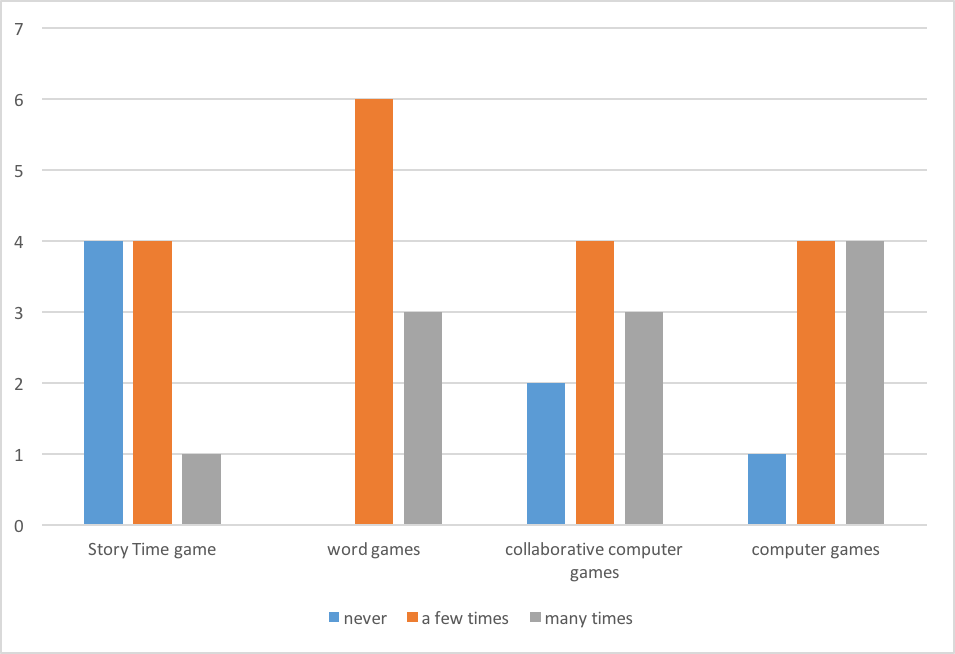
\includegraphics[width=0.4\textwidth]{demographics.png}
\caption{Interview Participants Previous Experience With Games}
\label{fig:demographics}
\end{figure}

\subsubsection{Interview Question Responses}
After analyzing the responses to the interview questions, we categorized the answers into nominal data. Appendix~\ref{apx:interview-responses} presents the summarized results in tabular format. 

From the responses gathered from the interviews, we noticed some interesting findings. First and foremost, we found that the participants prefer a time limit to be present, as this quote from \textit{Apollo} shows: \thinspace \thinspace
``\textit{... I think it [time limit] would add an element of pressure to the game, and you would not sort of be sitting there waiting for someone to come up with the perfect sentence... especially for the first [tiled] version if you're having to write your own stuff. Like waiting for someone to concoct their own thing, it would definitely get passed around really quick, and that would be kinda… it would imitate more the live version. Like if you're taking off the Sociables version where everyone is going around in a circle it would better emulate that. If you were doing the second version uhmm… you could have an even shorter time limit. That it's like, you just have to take your first instant reaction, and that could be cool too. You could make a really fast game like that.}'' \thinspace \thinspace  For the same question, \textit{Dionysus} mentions the difference of having a time limitation for remote games over in-person digital games. He says \thinspace \thinspace ``\textit{If you're playing alone on the internet (with random people) then yes. You would want it to be a faster game. But if you're with your friends I would say you don't really need a time limit.}'' \thinspace \thinspace

Another adaptation to the new environment would be generating a random title to help players start as this quote from \textit{Demeter} shows: ``\textit{I like when the title is there, it kinda just helps get the game going… having a theme chosen for you}'' \thinspace \thinspace \textit{Athena} gave an interesting suggestion about being given random titles that we had not thought of before: ``\textit{In a game scenario, I think to be able to re-generate the random title, maybe a maximum of 3 times, will be cool. The 3rd time you'll just have to go with that one.}'' \thinspace \thinspace

\subsubsection{Environmental study}
For the environmental study, we watched the participants while they were playing with both versions of the game to see their behaviour and reactions. For instance, they were seen laughing while reading the story during their turn for both the tiled and non-tiled version of StoryTime with Friends. This satisfies one of our main goals of ensuring the game is funny and entertaining. 

We also found that for the non-tiled version, some participants took up to two minutes to read the story and input their words, while others did not take as long (approximately 30 seconds). Due to the various reading abilities of players, as well as the length of the story, it is difficult for us to determine a viable time constraint for how long a player has to play their turn. Players will be able to take as much time as they need to read the story and input their words, but there will be a time constraint for how long it takes for them to return to the game, which begins as soon as they receive a notification letting them know it's their turn. This will ensure that the game is not ``stuck'' at one player's turn and will keep the game moving along. 


\subsection{Conceptual Design}
We have created a conceptual design, available in Appendix~\ref{apx:conceptual}, in order to assist in creating the user interface for the Minimal Viable Product, allowing us to easily notice any missing components in our game prior to the implementation. We will discuss the minimal viable product in detail in the Next Steps section. The conceptual design was planned out using an online, collaborative, diagramming tool called LucidChart. This tool makes it easy to create and share flowcharts, mockups, UML (Unified Modeling Language), mind maps and more.

\section{Discussion}
Contrary to our initial assumption that participants would enjoy the tiled prototype of StoryTime with Friends better than the non-tiled prototype, we found that 8 out of 9 participants actually favoured the non-tiled version. Based on the interview responses, the participants preferred having the freedom of inputting any words they liked, rather than being restricted to 6 sets of given words. 

\subsection{Not In Scope}
3 participants recommended a feature where an author of a game will be given a choice of a tiled or non-tiled version to play during the creation of a story. This feature may be considered for our final product, which is currently not in the scope of our project. Another feature that will not be in scope is the ability for players to join public games and read public stories. This is a feature that will be added to the final product, as 8 out of 9 participants agreed that they would participate in public games. Our Minimal Viable Product (discussed in Next Steps) and conceptual design will not take these features into consideration.


\section{Next Steps}

Since StoryTime with Friends is a project that is focused more on implementation rather than research, our team will be creating a Minimal Viable Product (MVP) in order to conduct further user testing. The MVP will take into consideration the information we gathered and analyzed from our first user testing on the prototypes discussed above. Each member in our team will perform a cognitive walkthrough of the MVP prior to the second user testing.

The MVP will be implemented as a web application, which when finalized, we intend to release as a Facebook game application. Due to the overwhelming majority of participants in our first user testing preferring the non-tiled prototype, our MVP will be implemented in this way. 

The purpose of the MVP is to decide on the features we have discussed for StoryTime with Friends and to determine whether they will be implemented into the final product. The MVP will be designed in a way that allow players to be distributed on their own computers while playing the game. This will introduce a more realistic approach in the user testing, in comparison to the first prototype, which forced the players to pass around a single computer. It is important to note, however, that the implementation of our final product is not in the scope of this project. We will instead discuss what we found from our user testing of the MVP and provide thorough documentation on what we believe the final product will consist of and why.

Our team has built the necessary platform in order to start the implementation process. The following are the tools we are using that allow us to collaborate on coding this application:

\begin{itemize}[leftmargin=.5in,nosep]
\item cPanel as web hosting control panel
\item phpMyAdmin, HeidiSQL and Sequel Pro as database management clients
\item GitHub allowing for version control and collaboration
\item PhpStorm by Jetbrains as our integrated development environment
\item PHP as server-side programming language
\item Apache as the web server
\item MySQL as relational database management server
\item HTML and CSS3 for front-end presentation
\item JavaScript programming language and jQuery library for front-end programming
\end{itemize}

\section{Acknowledgments}

We are extremely grateful to all the interview participants who accompanied us during our prototype evaluation. We would also like to give special thanks to our instructor, Prof. Margaret Storey, and teaching assistant, Eirini Kalliamvakou, who have provided invaluable assistance during the course of this project.

\nocite{*}
% REFERENCES FORMAT
% References must be the same font size as other body text.
\bibliographystyle{SIGCHI-Reference-Format}
\bibliography{bib}

\onecolumn
\createappendix{Progress Completed So Far}\label{apx:completed}

\begin{table}[h!]
\centering
\begin{tabular}{>{\raggedright}p{4cm}|>{\raggedright}p{6cm}|c}

\textbf{Project Milestone Met} &
\textbf{Description} &
\textbf{Date Completed} \\ \hline \hline

Written proposal &
Completed written proposal that describes what our project is about and the work that we will be doing this term. &
October 16, 2015 \\ \hline

Ethics application &
Ethics application and consent forms created in order to conduct interviews and prototype evaluation. &
October 19, 2015 \\ \hline

Finish prototype &
Finished creating two prototype versions of our game that will be tested by users. &
October 23, 2015 \\ \hline

Run prototype evaluation sessions &
Conducted two prototype evaluation sessions that involved participants playing with the prototypes. Interviewed participants to receive feedback and &
\makecell{October 26, 2015 \\ October 29, 2015} \\ \hline 

Analyzing data from prototype evaluation &
Transcribed the recorded interviews to analyze the data. Determined from the data which prototype version of the game and features the participants liked. &
October 27, 2015 \\ \hline

Finalize project requirements &
Discussed as a group what our project’s final requirements are and how we will be moving forward. &
October 30, 2015 \\ \hline

Conceptual design &
Conceptual design completed in order to assist the creation of our MVP. &
November 3, 2015 \\ \hline

\end{tabular}
\caption{Milestone Items Already Completed.}
\label{tab:met}
\end{table}


\createappendix{Milestones to be Completed}\label{apx:todo}

\begin{table}[h!]
\centering
\begin{tabular}{>{\raggedright}p{4cm}|>{\raggedright}p{6cm}|c}

\textbf{Project Milestone} & 
\textbf{Description} &
\textbf{Expected Date} \\ \hline \hline

Interim project report &
Complete interim report which describes our current work and the progress of the project. &
November 13, 2015 \\ \hline

Finalize MVP implementation &
The creation of a web application of the game will be completed. &
November 18, 2015 \\ \hline

Cognitive walkthrough of MVP implementation &
Each member of our team will conduct a cognitive walkthrough of the MVP to identify any usability issues. &
November 19, 2015 \\ \hline

Fix problems found after cognitive walkthrough &
Using the data collected from the cognitive walkthrough, we will improve and fix any problems of our MVP. &
November 20, 2015 \\ \hline

User testing (cooperative observation) of MVP followed by interviews &
Conduct our second round of user testing where participants will play the game using the MVP and be interviewed after. &
November 26, 2015 \\ \hline

Analyze and interpret interviews &
Using the data collected from the interviews, we will analyze and determine what the final product would have been like if we were doing the full implementation. &
November 27, 2015 \\ \hline

Final presentation &
Present to the class the work that we have completed. &
December 2, 2015 \\ \hline

Final report &
Final report describing in detail the work that we have done. &
December 5, 2015 \\ \hline

\end{tabular}
\caption{Planned Milestones to be Met.}
\label{tab:todo}
\end{table}



\createappendix{Demographic Questions}\label{apx:demographic}

\begin{enumerate}
\item Have you ever played Story Time game? (never, a few times, many times)

\item Have you ever played other types of word games? (never, a few times, many times)

\item Have you ever played collaborative computer games? (never, a few times, many times)

\item How frequent do you play computer games? (never, a few times a year, every month, every week, every day).

\end{enumerate}



\createappendix{Interview Questions}\label{apx:interview}

\begin{enumerate}
\item Did you prefer playing version 1 (input any words), or version 2 (choose from the given 
tiles of words) of the game? 

\item Did you like being given a random title for the story, or would you have preferred
inputting your own title?

\item This relates to the non-tiled version of the game. How many words do you think should 
be the maximum per turn?

\item Would you download and play our game with your friends (if it was free)? Why or why 
not?

\item We were thinking about limiting the amount of time the game takes, or the amount of 
time a player is allowed per turn by introducing a time limit. Do you think that the game 
should be time limited in some way? We would like to know your opinion for both the 
tiled version, and the non-tiled version of StoryTime.
\begin{itemize}
\item If so, how?
\end{itemize}

\item How many participants should partake in a game? (please answer in a range)

\item Do you think a chat feature would be useful for this game? Why or why not?

\item If you were allowed to play both public games and private games with friends, which one would you played more?

\item Were there any features that were missing which you would have liked to see from the 
gameplay?
\end{enumerate}




\createappendix{A Summary of Interview Question Responses}\label{apx:interview-responses}
\begin{tabular}{ | l | l | l | l | l | l | l | l | l | l | l | }
\hline
	  & Q1 & Q2 & Q3 & Q4 & Q5 & Q6 & Q7 & Q8 & Q9 \\ \hline
	Athena & non-tiled & Random Title & 4.5 & No & Yes & 3-5.5 & Maybe & Both & No \\ \hline
	Dionysus & non-tiled & Random Title & 3.5 & Yes & Mixed & 4-8 & Maybe & Both & Yes \\ \hline
	Hephaestus & non-tiled & Mixed Opinions & 4.5 & Yes & Yes & 2-10 & Yes & Both & No \\ \hline
	Demeter & non-tiled & Random Title & 6 & Yes & Yes & 4-8 & Maybe & Both & Yes \\ \hline
	Apollo & non-tiled & Random Title & 8 & Yes & Yes & 5-15 & No & Public Games & Yes \\ \hline
	Artemis & non-tiled & Random Title & 4 & Yes & Yes & 4-5 & No & Public Games & Yes \\ \hline
	Hades & non-tiled & Input own title & 5 & Yes & Mixed & 4-8 & Maybe & Public Games & Yes \\ \hline
	Aphrodite & tiled & Random Title & 4 & Yes & Yes & 4-6 & Maybe & Both & No \\ \hline
	Ares & non-tiled & Input own title & 5 & Yes & Yes & 3-6 & Yes & Family & No \\ \hline
\end{tabular}




\createappendix{Risks And Limitation}\label{apx:risks}

% This can be changed to a single column table with \begin{table}[h!] followed by \small,
% but it becomes REALLY small.
% Alternatively, move this around when the document is complete to get it on the top of the right page.
\renewcommand{\arraystretch}{1.5} %Add vertical padding
\begin{table}[h!]
%\small Un-comment this if switching to single column table
\centering
\begin{tabular}{ c | >{\raggedright}p{4cm} | c | c | >{\raggedright}p{5cm} | >{\raggedright\centering}p{2cm} l}
\textbf {No.} & 
\textbf{Risk Description} & 
\textbf{Probability} & 
\textbf{Impact} & 
\textbf{Planned Mitigation} & 
\textbf{Status} & \\ \hline \hline

1. &
Failure of translating the game in a way that is well-adapted to the new environment (online vs in-person) &
Medium &
High &
Interview our target audience in the design phase to find out what functionality and features they would be looking for in a game, considering the change in environment &
In progress & \\ \hline

2. &
Extremely diverse data as a result of high diversity in participants preferences and backgrounds &
Medium &
High &
Interview our target audience in the design phase to find out what functionality and features they would be looking for in a game, considering the change in environment &
Successfully overcome & \\ \hline

3. &
Proposing interview questions in a way that leads to biased answers &
Medium &
Medium &
Iteratively practice the interview and revise questions to reduce the chance of receiving biased responses &
Successfully overcome & \\ \hline


4. &
Participants responding to our questions while they don’t have enough information about the game &
Medium &
High &
Describing the game to participants, as well as, letting them play with a prototype before we ask them questions &
Successfully overcome & \\ \hline

5. &
Possible differences between the prototype with the actual application including environment differences (remote/face-to-face) and gameplay ones &
High & 
High &
Although we tried to simulate the remote/asynchronous environment by introducing some features, but this risk remains as a limitation to our project. &
Impact reduced - not overcome & \\ \hline

6. &
Difficulty of gathering many participants at the same time and location &
Medium &
Medium &
Breaking the interview into 2 sessions and inviting more potential participants &
Successfully overcome & \\ \hline

7. &
Failure in conducting the MVP due to lack of time &
Medium &
High &
Participation of all group members in development, preparing a multi-tier development framework to enable parallel team development &
To be overcome & \\ \hline

8. &
Maintenance – bugs, performance issues, etc. &
Medium &
Medium &
Regularly test the application for any usability, performance, and security issues, and update accordingly. &
To be overcome & \\ \hline

9. &
User experience – having usability issues for users &
Medium &
Medium &
Survey our target audience after the product launches to determine whether they are satisfied and ways we can improve. &
To be overcome & \\
\end{tabular}
\smallskip
\caption{Risks and Potential Limitations to be Faced.}
\label{tab:risks}
\end{table}


\createappendix{Conceptual Design}\label{apx:conceptual}


\begin{figure}[h!]
\centering
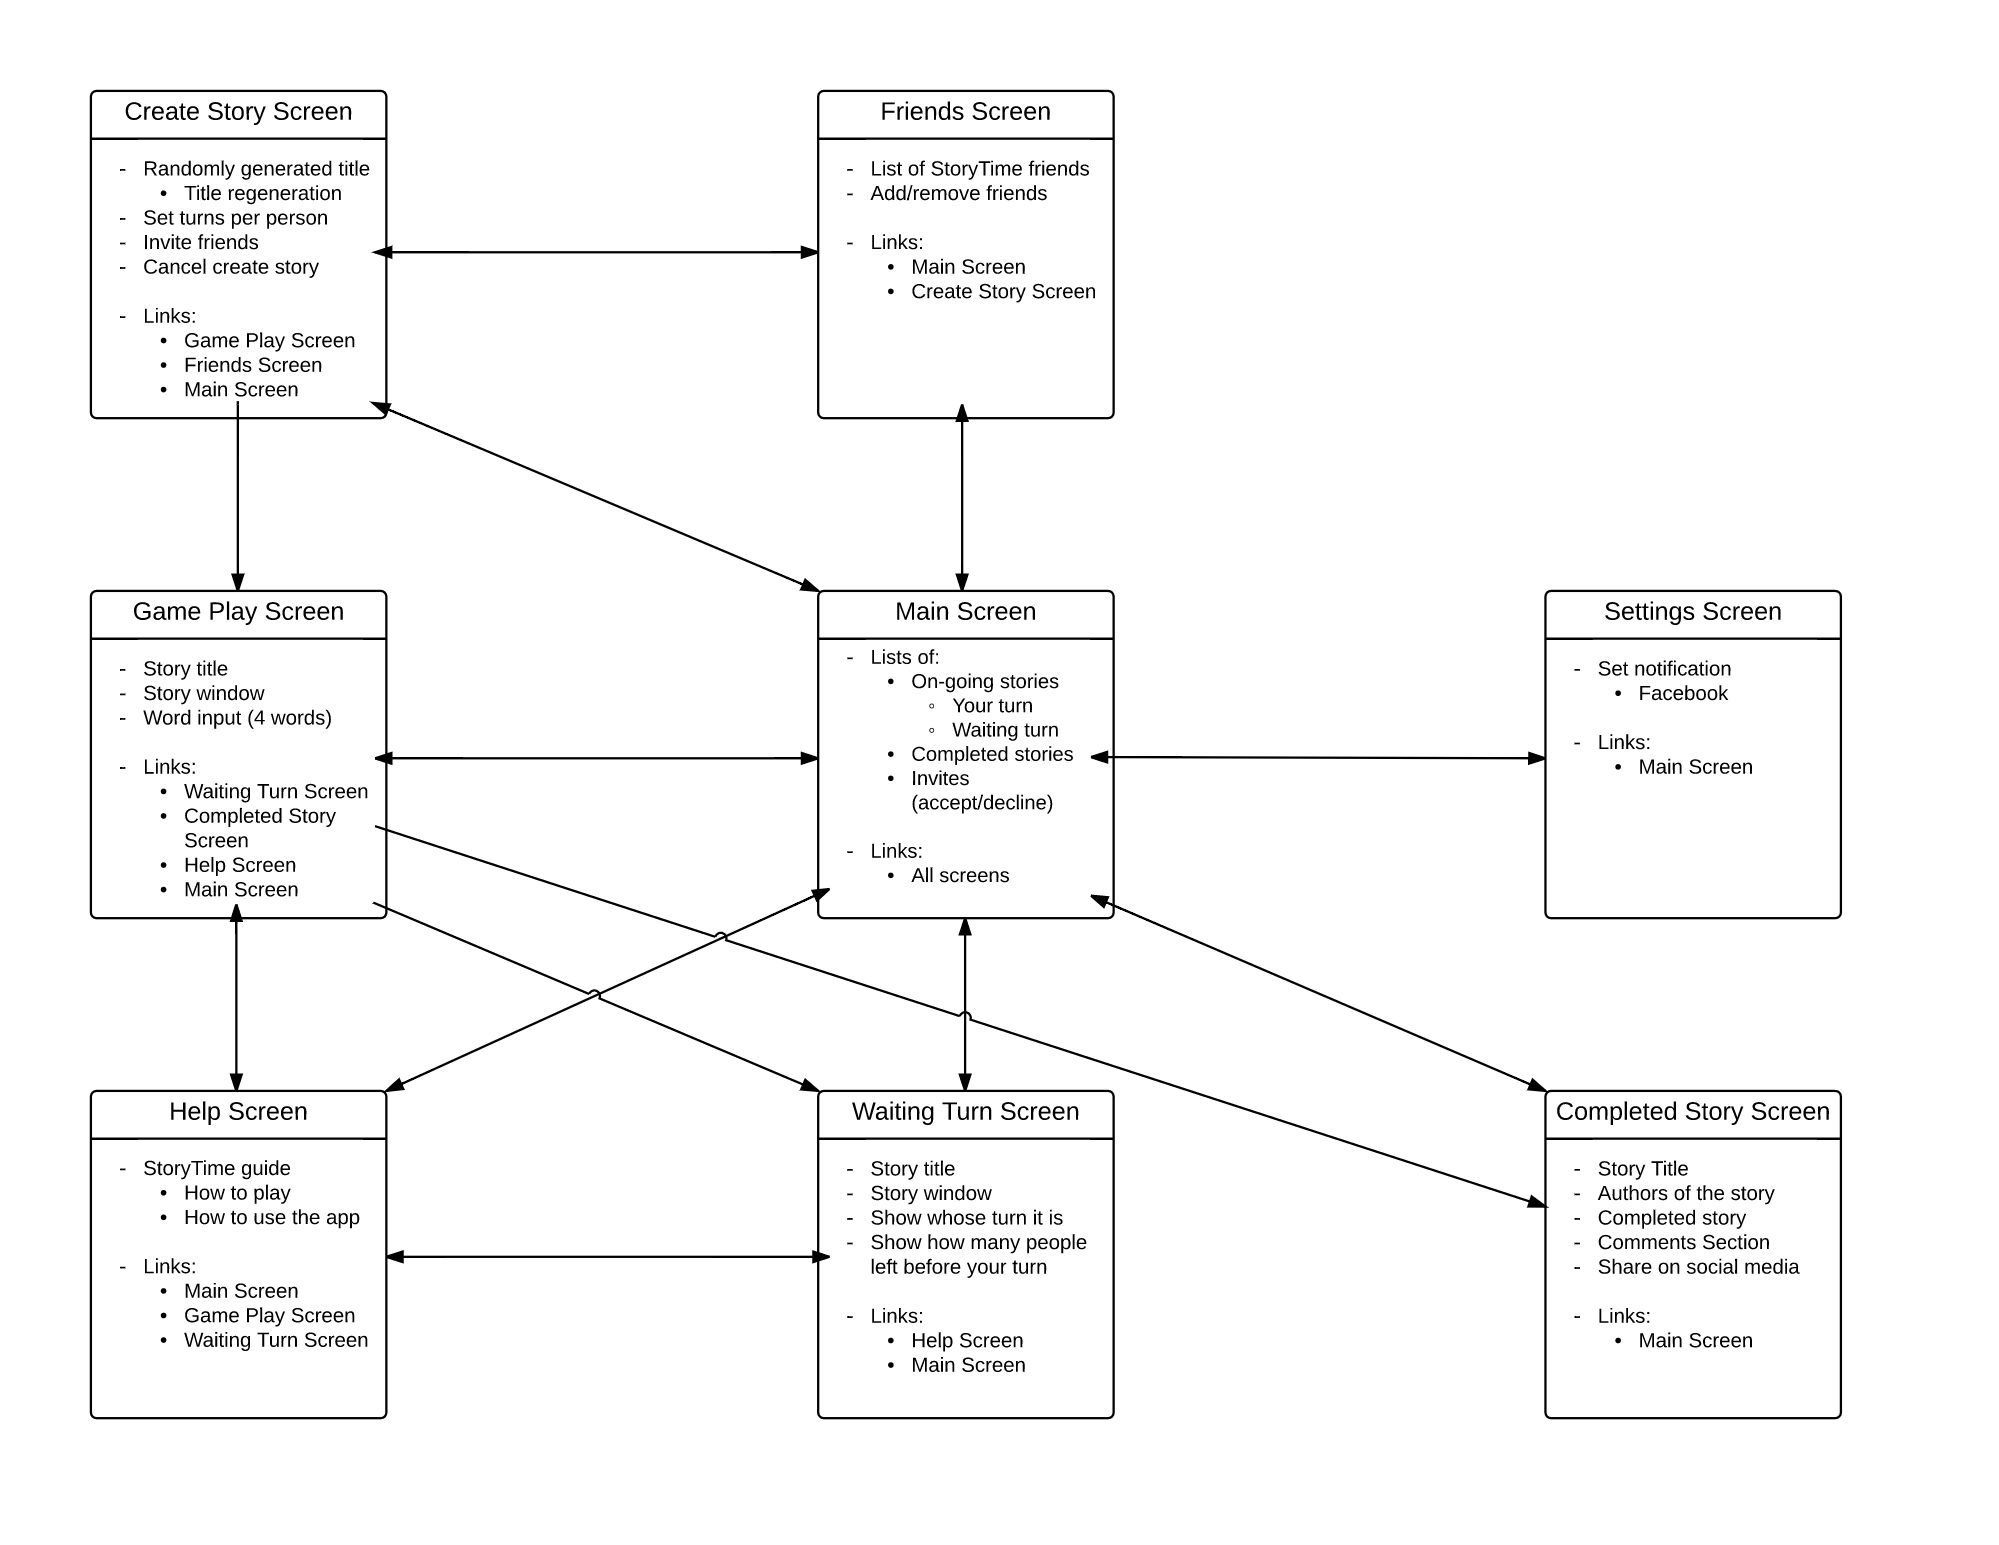
\includegraphics[width=\linewidth]{image00.png}
\caption{Conceptual Design for StoryTime With Friends}
\label{fig:conceptual}
\end{figure}



\end{document}

%%% Local Variables:
%%% mode: latex
%%% TeX-master: t
%%% End:
